\chapter{Implementierung}
\label{chap:Implementierung}

Die Anwendung RoCoVoMo wird in der Programmiersprache Java geschrieben und verwendet diverse Frameworks, die im folgenden kurz beschrieben werden:

\begin{itemize}
\item \textit{\gls{OSGi}}: Erm\"oglicht die Aufteilung der einzelnen Komponenten der Anwendung in sogenannte \textit{Bundles} oder Module die getrennt voneinander verwendet werden k\"onnen
\item \textit{jahmm}: Liefert alle Algorithmen und Komponenten, die zur Erstellung von \glspl{HMM} ben\"otigt werden
\item \textit{jnect}: Dient als Schnittstelle zwischen Kinect, Kinect SDK for Windows und der Java-Anwendung
\item \textit{lwjgl}: Erm\"oglicht die Verwendung von drei dimensionalen Grafiken der OpenGL Bibliothek
\end{itemize}

Dar\"uber hinaus wird die gesamte Java-Anwendung innerhalb der \gls{Eclipse} \gls{IDE} entwickelt und auf der aktuellen Juno 4.2 Plattform umgesetzt. Die Anwendung selbst wird in Form einer \gls{RCP} entwickelt und damit das \gls{OSGi} Framework von Eclipse, \gls{Equinox}, verwendet.
\newline
Im Folgenden werden die einzelnen Bestandteile der Anwendung n\"aher beschrieben.

\section{Architektur --- Design}
Seit den Arbeiten an der Anwendung f\"ur den ersten Teil der Arbeit wurde das Design und die Architektur der Anwendung nochmals \"uberarbeitet. Abbildung~\ref{fig:architecture} zeigt den aktuellen Stand der Anwendung.

\begin{figure}[htb]
\centering
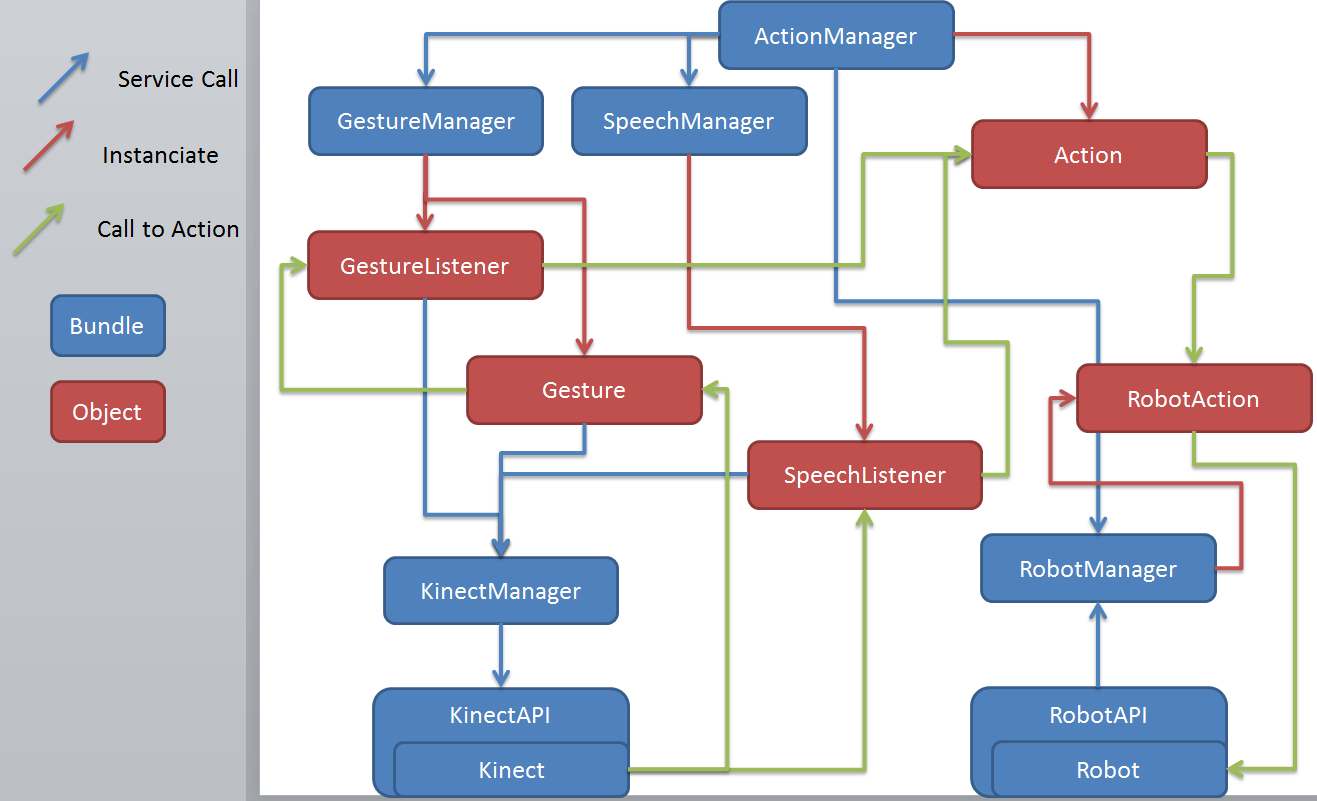
\includegraphics[width=0.8\textwidth]{img/impl/architecture.png}
\caption[Architekturdiagramm der Anwendung RoCoVoMo]{Architekturdiagramm der Anwendung RoCoVoMo}
\label{fig:architecture}
\end{figure}

Die mit der Farbe Blau markierten Elemente stellen sogenannte \gls{OSGi}-Bundles dar. Dabei handelt es sich vereinfacht gesprochen um einen Container, der eine bestimmte Logik beziehungsweise Fachlichkeit abdeckt und modular verwendbar ist. In der Anwendung RoCoVoMo werden mehrere solcher Bundles verwendet, die im Folgenden weiter beschrieben werden. Mit Rot markierte Elemente sind Java Klassen, die als Objekte innerhalb der Bundles verwendet werden.

\subsection{ActionManager}
In einer sogenannten \textit{Managerklasse}, in diesem Fall dem \textit{ActionManager} werden alle Aktionen verwaltet, die innerhalb der Anwendung ausf\"uhrbar sind. Die Managerklasse f\"uhrt dabei selbst keine Fachlichkeit aus, sondern delegiert diese an die darin verwalteten Objektinstanzen weiter, hier den einzelen Aktionen und ebenso an damit verbundene Bundles, hier \textit{GestureManager}, \textit{SpeechManager} und \textit{RobotManager}.
\newline
Diese Aufteilung erm\"oglicht es, Aktionen flexibel in die Anwendung zu integrieren, abzu\"andern oder gar zu l\"oschen. Weiter ist durch die loose Verbindung \"uber sogenannte \textit{Service Calls}, zum Beispiel des GestureManagers keine Abh\"angigkeit zu darin verwalteten Gesten vorhanden. Die einzige Verbindung zwischen Gesten und Aktionen findet im GestureListener statt, hierzu sp\"ater mehr.
\newline
Gleiches gilt f\"ur Sprache und der Roboteransteuerung.

\subsubsection{Action}
Die \textit{Action} ist so konzipiert, dass sie nicht direkt von einem Robotertyp abh\"angig ist. Diese Design erm\"oglicht sogar den relativ einfachen Umbau der Anwendung und Einsatz eines alternativen Robotermodells zum Lego NXT.
\newline
Wird eine Aktion ausgef\"uhrt, so ruft diese weiter die \textit{RoboterAction} aus, die die weitere Steuerung des Roboters \"ubernimmt, bisher der Lego NXT. Aufgerufen wird dieses Objekt von den Objekten \textit{GestureListener}, und \textit{Speechlistener}.

\subsection{GestureManager}
\textit{GestureManager} verwaltet alle in der Anwendung verf\"ugbaren Gesten. Dabei existiert pro \textit{Gesture}-Objekt ein \textit{GestureListener}.

\subsubsection{GestureListener}
\textit{GestureListener} liest Kinectinformationen aus und gleicht diese mit den \glspl{HMM} ab. Dabei werden \"uber spiezelle \textit{Recognizer}-Klassen, die Kinectdaten als HMM-Sequenzen eingelesen und Wahrscheinlichkeitsauswertungen im \gls{HMM} die richtige Geste erkannt und das entsprechende \textit{Gesture}-Objekt in Folge ausgef\"uhrt.

\subsubsection{Gesture}
\textit{Gesture} beinhaltet zahlreiche Meta-Informationen \"uber die entsprechende Geste und ist \"uber einen \textit{Actioncall} mit dem zugewiesenen \textit{Action}-Objekt verbunden. Wird das Gesture-Objekt vom Listener ausgef\"uhrt, so ruft Gesture diese Aktion auf.

\subsection{SpeechManager}
\textit{SpeechManager} verwaltet alle Sprachbefehle. Da Sprachbefehle bereits innerhalb der Kinect SDK integriert sind, und dieser lediglich \"uber String-Objekte und der entsprechenden Sprache hinzugef\"ugt werden m\"ussen, wurde darauf verzichtet ein gesondertes Objekt {Speech} zu modellieren, da dieses ledigliche die String Information enthalten w\"urde. Diese Daten sind im \textit{SpeechListener} hinerlegt.

\subsubsection{SpeechListener}
\textit{SpeechListener} f\"uhrt, sobald ein Sprachbefehl von der Kinect erkannt wurde, das entsprechende \textit{Action}-Objekt aus.

\subsection{KinectManager}
\textit{KinectManager} verwaltet die Verwendung von und den Datenaustausch mit der Kinect. Dieser wird von den Objekten \textit{GestureListener}, \textit{Gesture}, und \textit{SpeechListener} \"uber Service Calls aufgerufen.
\newline
Durch den Manager wird die KinectAPI und darin enthaltene Kinect f\"ur alle Teilnehmer sichtbar und dadurch kann ohne direkte Abh\"angigkeiten auf die Kinectinformationen zugegriffen werden.

\subsection{RobotManager}
\textit{RobotManager} verwaltet die Verwendung der RobotAPI und des darin enthaltenen Roboters. Bisher wird dadurch der Lego NXT verbunden. Durch diese Architektur ist jedoch auch m\"oglich weitere Robotermodelle in die Anwendung RoCoVoMo zu integrieren und weitere Abh\"angigkeiten zu erhalten.
\newline
Der Manager verwaltet weiterhin die Objekte \textit{RobotAction}, die dann aber je nach Robotermodell individuell geschrieben werden m\"ussen, da diese direkt auf die Roboter \gls{API} zugreifen, und diese sich von Modell zu Modell unterscheiden kann.

\section{Trainingsmodul}

\section{Kinect-Modul}

\section{Roboterinterface}